%************************************************
\chapter{Phylogenetic Tree}
%************************************************
\section{Objective}
Use genetic information to find the phylogenetic tree of given species.

\section{Requirements}
	\begin{enumerate}
		\item Computer with Mac/Windows/Linux
		\item Internet Access
		\item Phylip from \url{http://evolution.gs.washington.edu/phylip/getme.html}
		\item Treeview from \url{http://taxonomy.zoology.gla.ac.uk/rod/treeview.html}
		\item Clustal from \url{http://www.clustal.org/download/current/} (for windows use \url{clustalx-2.1-win.msi})
		\item mRNA data from \url{http://www.ncbi.nlm.nih.gov/} of the coding region only (this is specified on the page) for the following \label{tree_source}
		\begin{enumerate}
			\item rohu
			\item gonius
			\item kontius
			\item fimbriatus
			\item bata
		\end{enumerate}
	\end{enumerate}

\section{Brief Theory}
	The basic essence of this experiment hinges on the fact that there are coding and non coding regions in the DNA. The non-coding region can accumulate mutations over time without affecting the individual too much. However, the non-coding region can't tolerate high levels of divergence since that's closely related to the Darwinian fitness of the organism. It is for this reason, that we, to compare relatedness of species, use the coding region, which is easiest to obtain from the m-RNA data. We look at a specific protein's, viz. the Growth Hormone's m-RNA data in various species and compare them. 
	\par
	The non-coding region helps us establish, given two sets of species with equal relatedness, which had a common ancestor closer in the past.

\section{Procedure}
	\begin{enumerate}
		\item The data downloaded in accordance with \autoref{tree_source} and put in the format given in \autoref{tree_sourcefile} using any text editor (I used Sublime Text) and saved it, as say, `input.txt'. 
		\item ClustalX 
		\begin{enumerate}
			\item Now opened this file in ClustalX (the instructions may be biased towards windows henceforth for unavoidable reasons)
			\item \texttt{Selected Alignment -> Output Format}, and in the dialogue box checked \texttt{PHYLIP} format.
			\item Then, selected \texttt{Alignment -> Do Complete Alignment}, selected the right location and hit okay.
			\item Copied the \texttt{PHYLIP} file, wherever it was chosen to be created in the previous step, to the \texttt{exe} folder of \texttt{phylip-3.69}, renamed to \texttt{infile}, without any extension.
		\end{enumerate}
		A screenshot's given in \autoref{clustal}

		\item Phylip 
		\par
		This is a collection of executable files, which expect a file named input and create a file named output, on the basis of the parameters specified by the user, when the program is executed. \footnote{The last program produces a file named \texttt{outtree}} We will use the outputted files as inputs from one program to the next. Below is an ordered list of programs and the parameters to be specified, to be used sequentially (redundancy is used for emphasis). 
		\begin{enumerate}
			\item \texttt{seqboot}
			\item \texttt{dnapars}
			\begin{enumerate}
				\item M (Analyse multiple data set)
				\item D (Multiple Data sets, not multiple weights)
				\item 30 (Number of Data Sets)
				\item 1/3/7 (Enter Seed, input any odd number)
				\item 500	(Number of times to Juggle)
			\end{enumerate}
			You could also modify the number of trees to save.
			\item \texttt{consense}			
		\end{enumerate}
		\item Treeview
		\par
		Use the \texttt{outtree} file created in the previous step and obtain the required tree.
		A screenshot's given in \autoref{tree}
	\end{enumerate}

\begin{lstlisting}[float,caption=Format of the source file,label=tree_sourcefile]
>rohu
atggctagagcattagtgctgttgtcggtggtgctggttagttt....
>gonius
atggctagagcattagtgctgttgtcggtggtgctggttagtct....
>kontius
atggctagagcattagtgctgttgtcggtggtgctggttagttt....
>fimbriatus
atggctagagcattagtgctgttgtcggtggtgctggttagttt....
>bata
atggctagagcattagtgctgttgtcggtggtgctggttagttt....
\end{lstlisting}

\begin{figure}[bth]
	\begin{center}
		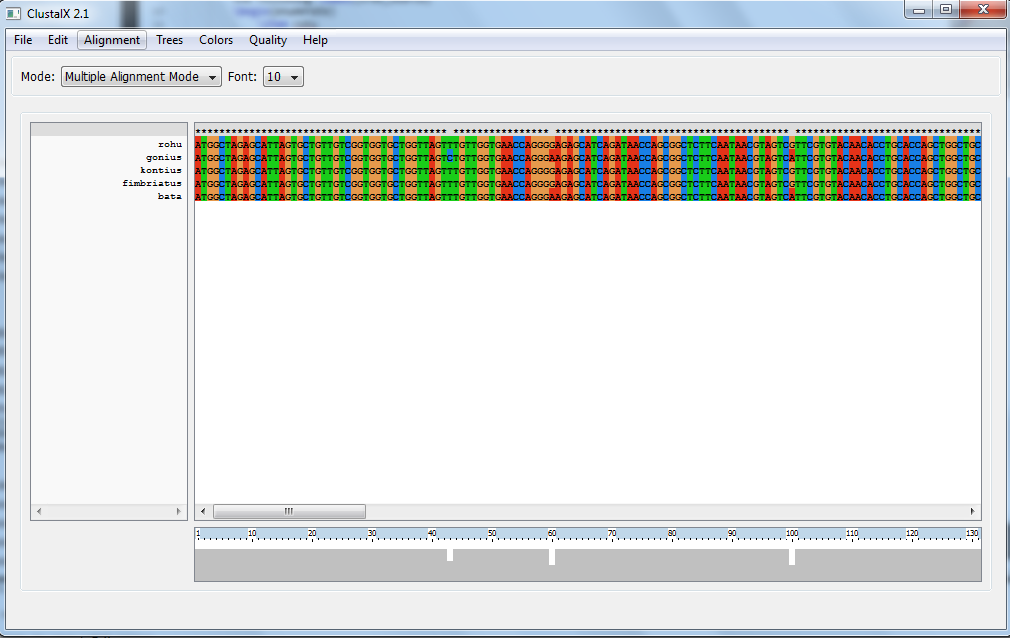
\includegraphics[width=1.1\linewidth]{gfx/clustal}
	\end{center}
\caption[ClustalX]{ClustalX}
\label{clustal}
\end{figure}

\begin{figure}[bth]
	\begin{center}
		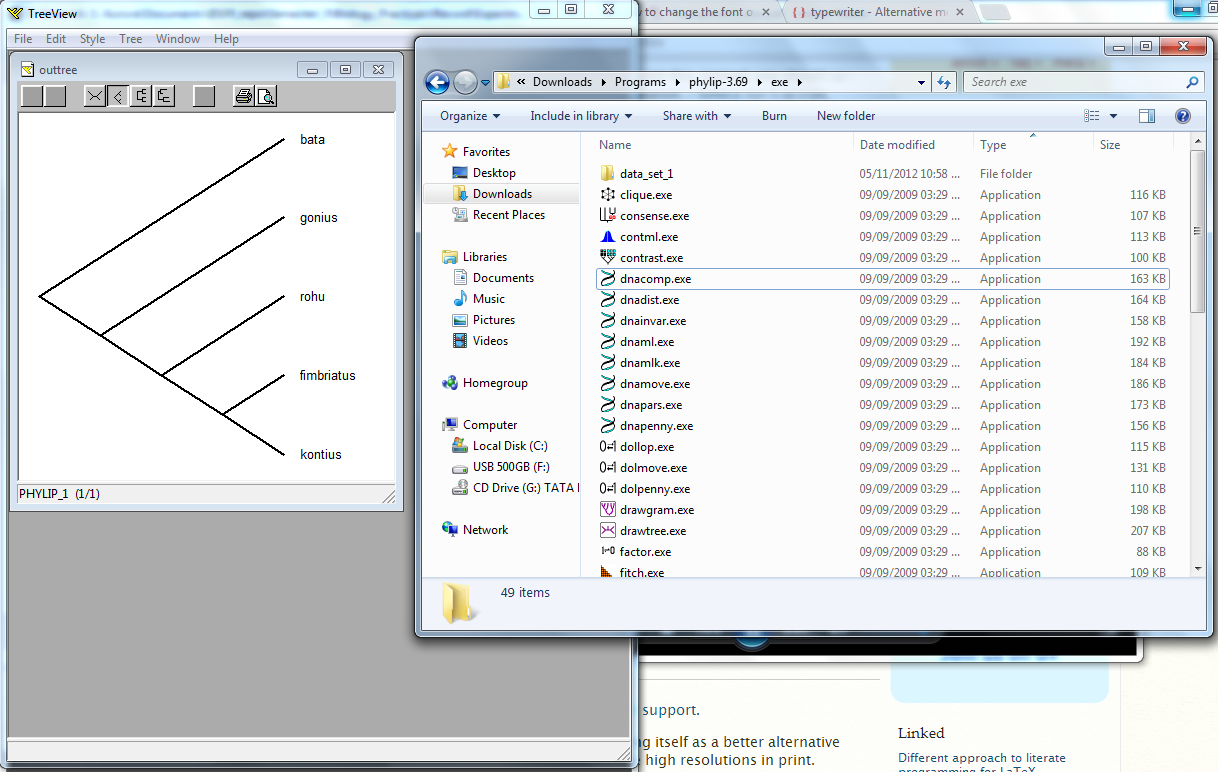
\includegraphics[width=1.2\linewidth]{gfx/tree}
	\end{center}
\caption[Treeview and Phylip]{Treeview and Phylip}
\label{tree}
\end{figure}


\section{Acknowledgement}
	I am thankful to my friend, Mr. Vivek Sagar, for taking notes while the experiment was being performed. I sincerely express my gratitude for Dr. Sanjay Mandal, who introduced us to this aspect of Biological analysis.